% Main-text figure -- the core of the VCF Core model, as VCF-RDFizer emits it.
% A reduced view of vcf-core-classes.tex (Supplementary Figure S1): the same
% classes, colours, and lanes, without subclasses, value items, or property names.
% Solid arrows read "contains" (the ownership the policy plug-in follows when it
% withholds a resource); dashed arrows are references between layers.
% Standalone TikZ source; build with: pdflatex vcf-core-minimal.tex -> vcf-core-minimal.pdf
% Drawn within the journal text width (372pt, about 13.1 cm) so it is included unscaled.
\documentclass[border=1pt]{standalone}
\usepackage[T1]{fontenc}
\usepackage{helvet}
\renewcommand{\familydefault}{\sfdefault}
\usepackage{tikz}
\usetikzlibrary{arrows.meta,positioning,calc,backgrounds}

% Model palette, shared with the other model figure and kept apart from every hue
% in the pipeline figure (vcf2rdf-v3.tex): brown file, raspberry header, olive
% record, indigo samples, and jade for the condensed profile.
\definecolor{chdr}{HTML}{F8E0EC}  \definecolor{chdrd}{HTML}{A3296A}
\definecolor{crec}{HTML}{EDF0D5}  \definecolor{crecd}{HTML}{66761A}
\definecolor{csmp}{HTML}{E3E2F4}  \definecolor{csmpd}{HTML}{3E3B98}
\definecolor{ccon}{HTML}{DCF2E9}  \definecolor{ccond}{HTML}{1B8A62}
\definecolor{cfile}{HTML}{EFE6DC} \definecolor{cfiled}{HTML}{7B5A38}
\definecolor{cband}{HTML}{F7F7F7}

\begin{document}
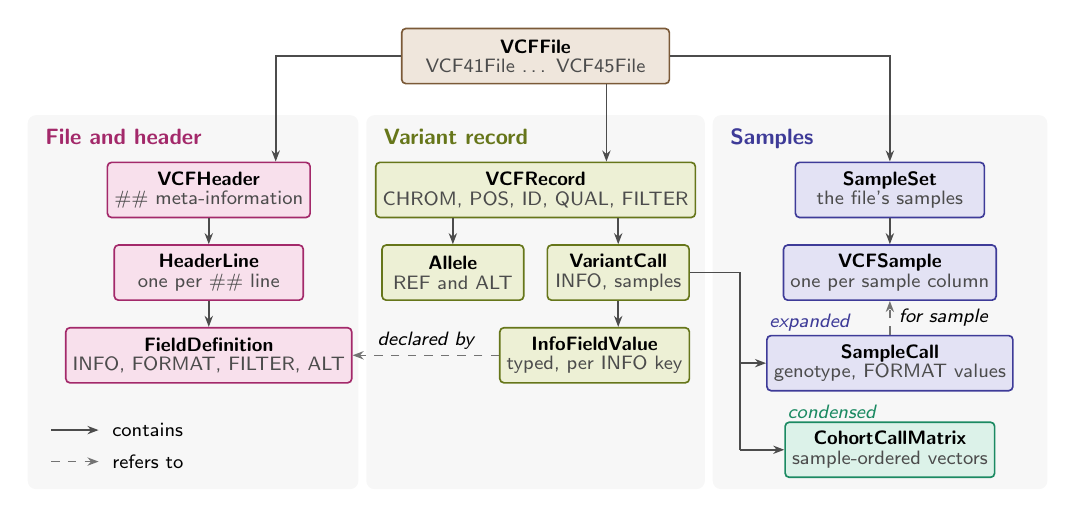
\begin{tikzpicture}[
  font=\scriptsize,
  cls/.style={draw, rounded corners=1.5pt, line width=0.6pt, align=center, inner sep=2.5pt,
              minimum height=0.7cm, minimum width=2.4cm},
  has/.style={-{Stealth[length=4pt]}, line width=0.6pt, draw=black!70},
  ref/.style={-{Stealth[length=4pt]}, line width=0.55pt, draw=black!55, dashed},
  p/.style={font=\scriptsize\itshape, fill=cband, inner sep=1pt},
  lane/.style={font=\footnotesize\bfseries\itshape, anchor=north west},
  prof/.style={font=\scriptsize\itshape, anchor=south west, inner sep=1pt},
]
\newcommand{\cl}[2]{\textbf{#1}\\[-1pt]{\color{black!70}#2}}

% ------------------------------------------------------------------ root
\node[cls, fill=cfile, draw=cfiled, minimum width=3.4cm] (file) at (6.45,0)
  {\cl{VCFFile}{VCF41File \dots\ VCF45File}};

% ------------------------------------------------------------------ file and header
\node[lane, text=chdrd] at (0.1,-0.8) {File and header};
\node[cls, fill=chdr, draw=chdrd] (hdr)  at (2.3,-1.7) {\cl{VCFHeader}{\#\# meta-information}};
\node[cls, fill=chdr, draw=chdrd] (line) at (2.3,-2.75) {\cl{HeaderLine}{one per \#\# line}};
\node[cls, fill=chdr, draw=chdrd] (def)  at (2.3,-3.8) {\cl{FieldDefinition}{INFO, FORMAT, FILTER, ALT}};

% ------------------------------------------------------------------ variant record
\node[lane, text=crecd] at (4.4,-0.8) {Variant record};
\node[cls, fill=crec, draw=crecd] (rec) at (6.45,-1.7) {\cl{VCFRecord}{CHROM, POS, ID, QUAL, FILTER}};
\node[cls, fill=crec, draw=crecd, minimum width=1.8cm] (allele) at (5.4,-2.75) {\cl{Allele}{REF and ALT}};
\node[cls, fill=crec, draw=crecd, minimum width=1.8cm] (call)   at (7.5,-2.75) {\cl{VariantCall}{INFO, samples}};
\node[cls, fill=crec, draw=crecd] (info) at (7.2,-3.8) {\cl{InfoFieldValue}{typed, per INFO key}};

% ------------------------------------------------------------------ samples
\node[lane, text=csmpd] at (8.8,-0.8) {Samples};
\node[cls, fill=csmp, draw=csmpd] (set)    at (10.95,-1.7) {\cl{SampleSet}{the file's samples}};
\node[cls, fill=csmp, draw=csmpd] (sample) at (10.95,-2.75) {\cl{VCFSample}{one per sample column}};
\node[cls, fill=csmp, draw=csmpd] (scall)  at (10.95,-3.9) {\cl{SampleCall}{genotype, FORMAT values}};
\node[cls, fill=ccon, draw=ccond] (matrix) at (10.95,-5.0) {\cl{CohortCallMatrix}{sample-ordered vectors}};

% ------------------------------------------------------------------ contains
% Arrows from the file enter the header and record boxes right of the lane titles.
\draw[has] (file.west) -| ($(hdr.north)+(0.85,0)$);
\draw[has] ($(file.south)+(0.9,0)$) -- ($(file.south |- rec.north)+(0.9,0)$);
\draw[has] (file.east) -| (set.north);
\draw[has] (hdr) -- (line);
\draw[has] (line) -- (def);
\draw[has] (rec.south -| allele.north) -- (allele.north);
\draw[has] (rec.south -| call.north) -- (call.north);
\draw[has] (call.south) -- (call.south |- info.north);
\draw[has] (set) -- (sample);
% one call holds its samples in either profile
\draw[line width=0.6pt, draw=black!70] (call.east) -- (9.05,-2.75) -- (9.05,-5.0);
\draw[has] (9.05,-3.9) -- (scall.west);
\draw[has] (9.05,-5.0) -- (matrix.west);

% ------------------------------------------------------------------ references
\draw[ref] (info.west) -- node[p, above=1pt]{declared by} (def.east |- info.west);
\draw[ref] (scall.north) -- node[p, right=2pt]{for sample} (sample.south);

% ------------------------------------------------------------------ lanes, profiles, legend
\begin{scope}[on background layer]
  \fill[cband, rounded corners=3pt] (0,-0.75) rectangle (4.2,-5.5);
  \fill[cband, rounded corners=3pt] (4.3,-0.75) rectangle (8.6,-5.5);
  \fill[cband, rounded corners=3pt] (8.7,-0.75) rectangle (12.95,-5.5);
\end{scope}
\node[prof, text=csmpd] at (scall.north west) {expanded};
\node[prof, text=ccond] at (matrix.north west) {condensed};

\begin{scope}[shift={(0.3,-4.75)}]
  \draw[has] (0,0) -- (0.6,0);         \node[anchor=west] at (0.65,0) {contains};
  \draw[ref] (0,-0.4) -- (0.6,-0.4);   \node[anchor=west] at (0.65,-0.4) {refers to};
\end{scope}
\end{tikzpicture}
\end{document}
